\chapter{Definizione del quadro sperimentale}
\setcounter{section}{1}
Al principio i dati dovevano essere trattati con la stessa configurazione architetturale dei metadati, utilizzando il modello di \textit{publush/provider} e le sottoscrizioni sincrone e asincrone.\\

I lanci di configurazione che seguono hanno condotto verso un tipo di architettura differente per gestire la ridondanza del dato.\\
Dai risultati dei test \`{e} comprensibile la preferenza di un'altra scelta: utilizzare la stessa replicazione del metadato non \`{e} conveniente.\\

Inizialmente, \`{e} stato possibile notare che utilizzando Postgres, la scrittura di un dato su un database, apriva una connessione a un altro nodo inviandogli la copia del dato in modo sincrono. Questo causava lente prestazioni.\\
La libreria utilizzata scritta a codice, per cui veniva ridondata soltanto una copia, causava eccessivi rallentamenti.\\

Ci\`{o} ha portato a un cambiamento del codice, ottenendo in questo modo la configurazione attuale: il dato viene scritto in due database e le risposte di successo o eventuale fallimento, sono gestite direttamente da codice; \`{e} restituito un \verb"rollback" se la ridondanza non \`{e} effettuabile, in caso contrario \`{e} ritornato un \verb"commit" soltanto se entrambi i database hanno scritto la replicazione del dato.

\item 
\section{Dati del quadro sperimentale}
I dati sono stati ricavati dai \verb"log" di \textit{nginx}. \\
Nginx \`{e} un \textit{web server/reverse proxy} leggero ad alte prestazioni e fornisce in modo rapido i contenuti statici con un utilizzo efficiente delle risorse del sistema.\\
Ci\`{o} \`{e} interessante in quanto rende la misura maggiormente obiettiva. Di fatto i risultati non sono ottenuti da uno strumento "imparziale", al contrario da terze parti, quale ngnix che non sfavorisce n\`{e} favorisce.\\
Dai \verb"log" di nginx sono state prese in considerazione le \verb"PUT" dei \textit{chunk}. In particolar modo \`{e} stato necessario controllare il tempo di quando ogni pacchetto entra all'interno dello \textit{storage} a quando esce (tempo dato in \verb"ms"). Questo tempo \`{e} stato successivamente raggruppato al decimo di secondo.\\

I dati sono di fatto il numero dei pacchetti, ossia la frequenza di \verb"PUT" registrate da nginx, e il tempo impiegato da ogni dato.

\item
\section{Lanci di configurazione}
Per stabilire questa decisione architetturale sono stati esaminati vari lanci con configurazioni diverse.\\
In parte dei casi \`{e} stato influente, altre sono state peggiorative, fino a che non abbiamo ottenuto il risultato finale.\\ 
Esaminiamo i principali lanci di configurazioni che ci hanno portato a queste riflessioni.

\item
\subsubsection{Lancio di configurazione 1} 
Nel primo lancio \`{e} partecipe una singola istanza Postgres. \\
Non \`{e} presente nessuna copia di ridondanza. Questo rappresenta il caso ottimale, indubbiamente il migliore; tuttavia non ha vantaggi in quanto non ridonda i dati.\\
In aggiunta sono state aumentate il numero di connessioni a \verb"60" (invece che a \verb"40" come in tutti gli altri lanci di configurazione) arrivando in questo modo a ottenere \verb"133Mbit/sec".

\begin{center}
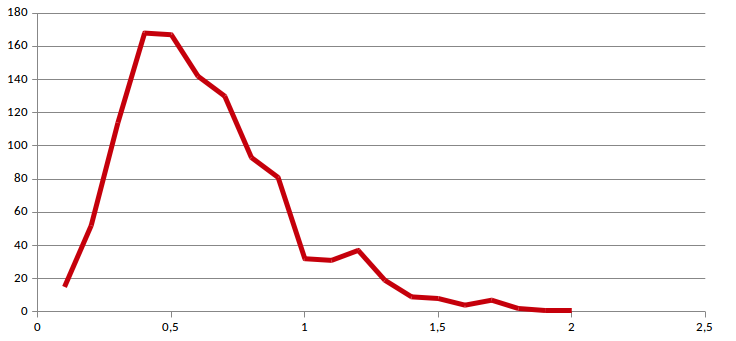
\includegraphics[scale=0.70]{img/round2.png}
\end{center}
\begin{figure}[htbp]
\caption{Singola istanza Postgres. Nessuna copia di ridondanza. \label{figura1.15}}
\end{figure}

\item
\subsubsection{Lancio di configurazione 2}
Questo lancio \`{e} stato utile in quanto \`{e} stato possibile scoprire che le connessioni non erano parallele ma sequenziali.\\
Le chiamate avvenivano per mezzo di una libreria scritta che per\`{o} non rendeva le connessioni parallele. Cos\`{i} facendo le connessioni per scrivere il dato erano sequenziali. Le connessioni erano di fatto aperte soltanto su richiesta e questo provoca un ritardo dei tempi essenziale.\\
Sono state configurate due sottoscrizioni sincrone e questo ha portato ad ottenere senza dubbi il caso peggiore.

\begin{center}
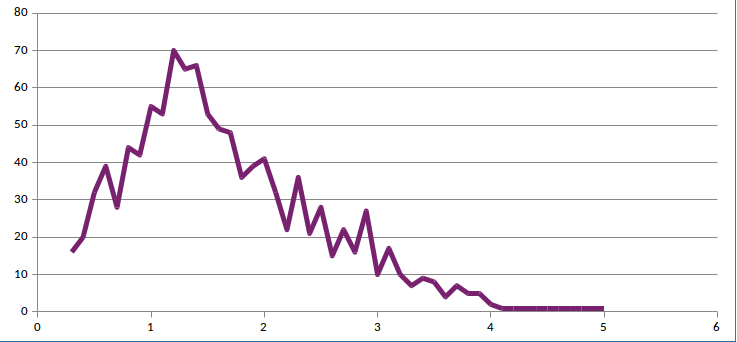
\includegraphics[scale=0.70]{img/round1b.png}
\end{center}
\begin{figure}[htbp]
\caption{Introdotte le \textit{foreign-table}. Scoperta del non parallelismo delle connessioni. \label{figura1.15}}
\end{figure}

\item
\subsubsection{Lancio di configurazione 3} 
In questo lancio sono state utilizzate pi\`{u} istanze Postgres, al fine di avere sottoscrizioni sincrone, altrimento avremo una sola sottoscrizione sincrona e tutte le altre asincrone.\\

In questo scenario sono mandati pi\`{u} di una copia per chunk usando sottoscrizioni asincrone.

\begin{center}
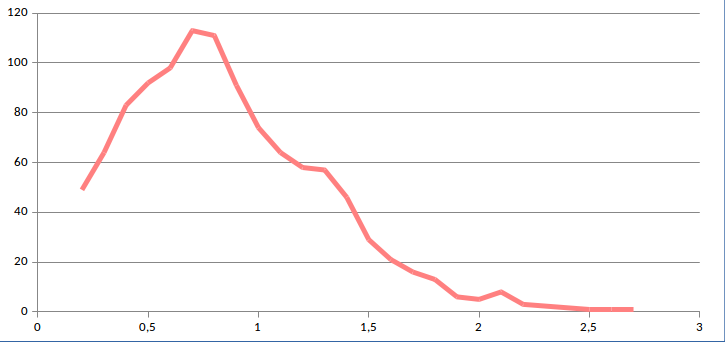
\includegraphics[scale=0.70]{img/round1.png}
\end{center}
\begin{figure}[htbp]
\caption{Pi\`{u} copie per chunk con sottoscrizioni asincrone. \label{figura1.15}}
\end{figure}

Il risultato ottenuto si trova in una posizione centrale rispetto ai due casi limite. Tuttavia la campana formata \`{e} ancora troppo larga per poter esser soddisfatti del risultato.

\begin{center}
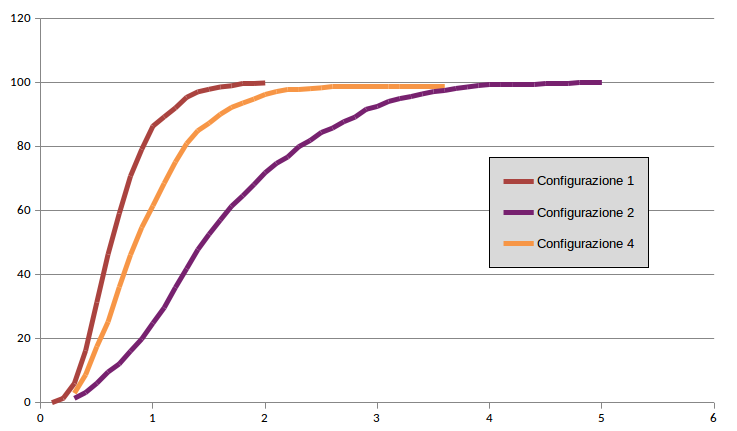
\includegraphics[scale=0.70]{img/comparison2.png}
\end{center}
\begin{figure}[htbp]
\caption{Risultato dei quattro lanci di configurazione \label{figura1.15}}
\end{figure}

\item
\subsubsection{Lancio di configurazione 4} 
Nella seguente configurazione sono state tolte le \textit{foreign-table}.\\
Le connessioni sono aperte in serie, mentre le \verb"PUT" sono in parallelo. Le connessioni non incidono eccessivamente.\\
Iniziano a rilevarsi miglioramenti, in quanto \`{e} presente un primo avvicinamento ai tempi della configurazione \verb"1", ossia quella ottimale.

\begin{center}
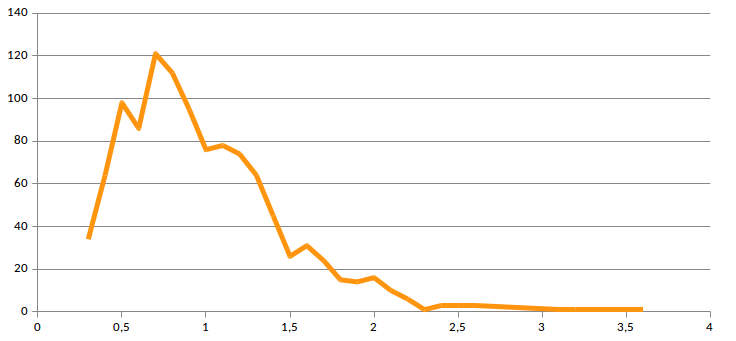
\includegraphics[scale=0.70]{img/round4b.png}
\end{center}
\begin{figure}[htbp]
\caption{Tolte le \textit{foreign-table}. Connessioni in serie e PUT in parallelo. \label{figura1.15}}
\end{figure}

I miglioramenti sono visibili dal confronto dei lanci di configurazione.

\begin{center}
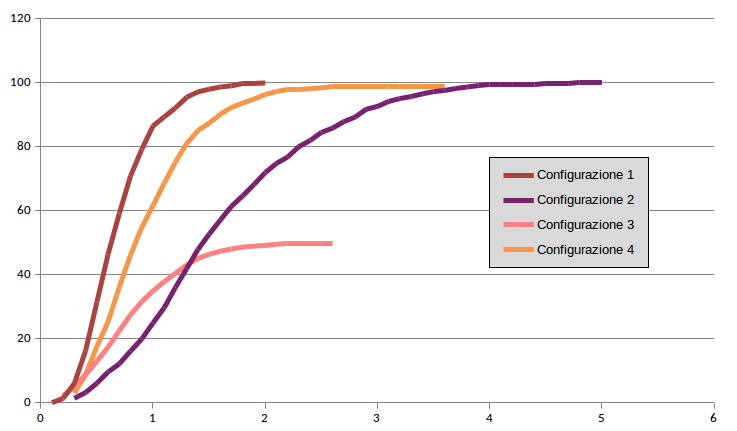
\includegraphics[scale=0.70]{img/comparison1.png}
\end{center}
\begin{figure}[htbp]
\caption{Risultato dei quattro lanci di configurazione \label{figura1.15}}
\end{figure}

\item
\subsubsection{Lancio di configurazione 5}
In questo ultimo lancio sono state tolte definitivamente le \textit{foreign-table}. Le \verb"PUT" sono in parallelo. \\
In aggiunta sono stati disabilitati i \verb"log" di Postgres e le connessioni sono aperte in parallelo. Pi\`{u} nello specifico, si aprono alcune connessioni in parallelo che scrivono sul database, senza attendere messaggi di successo su tutt gli altri database. \\
Si nota che \`{e} il risultato migliore ottenuto fino ad ora, anche se non totalmente impeccabile. Questo scenario \`{e} un compromesso ragionevole del caso ottimale, che tuttavia non garantiva la ridondanza del dato.\\
\`{E} possibile notare dalla curva che il sistema rallenta sotto \verb"80%", peggiorando solo per un \verb"20%" dei casi. \\
Ci\`{o} permette di concludere che la strategia di avere un solo database \`{e} vantaggioso per un punto di vista di performance. \\
Otteniamo in questo modo un'affidabile sicurezza in buoni tempi, arrivando a \verb"126Mbit/sec". 

\begin{center}
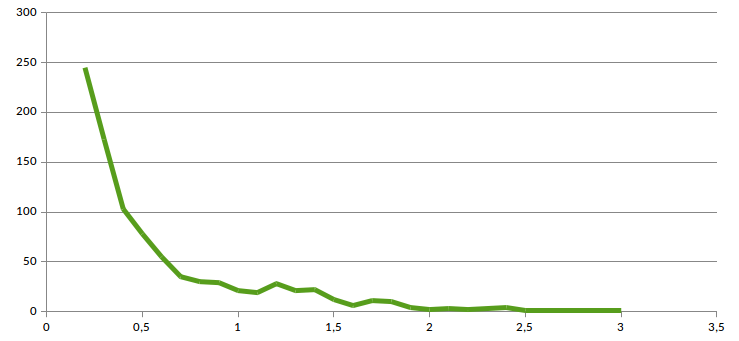
\includegraphics[scale=0.70]{img/round8c.png}
\end{center}
\begin{figure}[htbp]
\caption{Connessioni in parallelo e PUT in parallelo.) \label{figura1.15}}
\end{figure}

Il confronto totale ottenuto dai lanci di configurazione appena esaminati, restituisce il seguente grafico:

\begin{center}
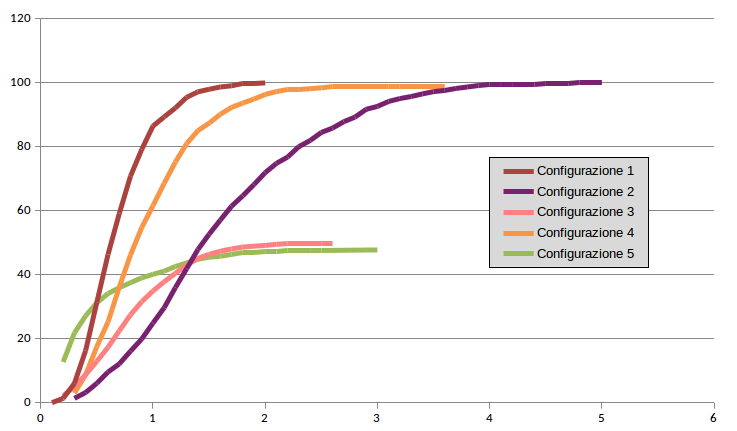
\includegraphics[scale=0.70]{img/comparison_tot1.png}
\end{center}
\begin{figure}[htbp]
\caption{Scenario globale dei lanci di configurazione) \label{figura1.15}}
\end{figure}

Segue un grafico che rappresenta la frequenza cumulata dello scenario globale, che corrisponde alla somma dei grafici precedentemente ottenuti su base \verb"100". In sostanza \`{e} pari alla percentuale.\\
Pi\`{u} \`{e} larga la campana descritta dalle linee, maggiormente la distribuzione \`{e} distesa.\\
Quando la campana \`{e} stretta, significa che quel comportamento \`{e} indice di un fattore rilevante.

\begin{center}
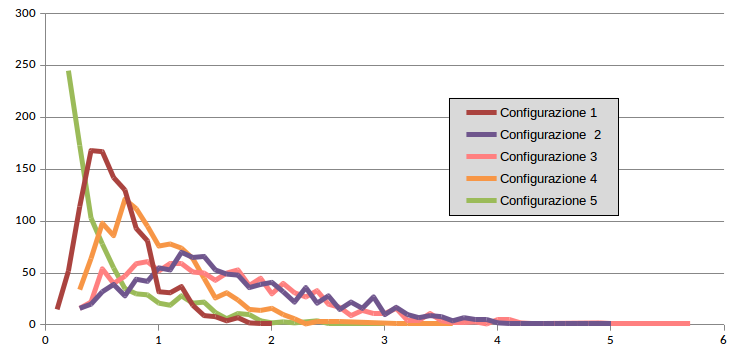
\includegraphics[scale=0.70]{img/comparison_tot2.png}
\end{center}
\begin{figure}[htbp]
\caption{Frequenza cumulata dello scenario globale) \label{figura1.15}}
\end{figure}

